\documentclass[12pt,a4paper]{article}
\pagestyle{plain}
\usepackage{fullpage}
\usepackage[english]{babel}
\usepackage{enumerate}

%equations
\usepackage[fleqn]{amsmath}
\numberwithin{equation}{section}

%figures
\usepackage[dvips]{graphicx}
\graphicspath{{./images/}}
\numberwithin{figure}{section}

%excercises
\newcounter{Exercise}
\setcounter{Exercise}{1}
\usepackage[dvipsnames]{xcolor}
\usepackage{framed}
\definecolor{shadecolor}{gray}{0.9}
\usepackage{caption}

%tables
\numberwithin{table}{section}

%specials
\usepackage{textcomp} %special (greek) characters as text
%\usepackage{pstricks} %
%\usepackage{ifthen} %
%\usepackage{calc} %


%document details
\author{N.G. Schultheiss \\ translated and adapted by K. Schadenberg}
\date{}
\title{Parabolic Mirrors}


\begin{document}
\maketitle

\section{Introduction}
This module `Parabolic Mirrors follows the module `Mirrors' and can lead to the module `Grinding Lenses' and `Telescopes'. When you completed all these modules you should be able to make your own telescope with the help of the module `Making your own telescope' and explain how it works. This module is more technical then the previous one because it focusses more on constructing a mirror then on the mathematics behind the process.

The following equations should be familiar:
\begin{align}
v &= \frac{\Delta s}{\Delta t} \\
a &= \frac{\Delta v}{\Delta t} \\
F &= m \cdot a \label{eq:newton2}
\end{align}
with $v$ velocity [m/s], $s$ location (space) in [m], $t$ time [s], $a$ acceleration [m/s$^{2}$], $F$ force [N], and $\Delta$ meaning change or difference, $\Delta s$ would therefore be displacement: $\Delta s = s_{end} - s_{start}$.

\section{A turning barrel}
When we pour a liquid into a turning barrel its surface will take the shape of a parabola. To explain this behaviour we first need to look at the forces involved. Let us draw a map of the circular motion of the barrel at different moments in time: $t_1$, $t_2$, $t_3$, and $t_4$.
\begin{figure}\begin{center}
\begin{picture}(0,0)%
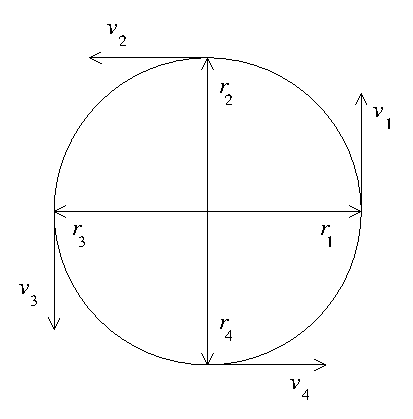
\includegraphics{location_xfig}%
\end{picture}%
\setlength{\unitlength}{4144sp}%
%
\begingroup\makeatletter\ifx\SetFigFont\undefined%
\gdef\SetFigFont#1#2#3#4#5{%
  \reset@font\fontsize{#1}{#2pt}%
  \fontfamily{#3}\fontseries{#4}\fontshape{#5}%
  \selectfont}%
\fi\endgroup%
\begin{picture}(2881,2925)(436,-1966)
\end{picture}%
\caption{The location of a turning object.}\label{fig:turning_object}
\end{center}\end{figure}

Using figure~\ref{fig:turning_object} we can determine the speed if we set the time required to complete one rotation at $T$. The distance travelled is easily calculated by dividing the circumference of the barrel by the duration of one rotation:
\begin{equation}
v= \frac{2 \pi r}{T} \label{eq:v_T}
\end{equation}
We can rearrange this into:
\begin{equation}
T= \frac{2 \pi r}{v} \label{eq:T_v}
\end{equation}

Figure~\ref{fig:turning_object} depicts places and allows us to calculate velocities. We can also make a figure depicting velocities to calculate accelerations, as we did in figure \ref{fig:turning_object_speed}.
\begin{figure}\begin{center}
\begin{picture}(0,0)%
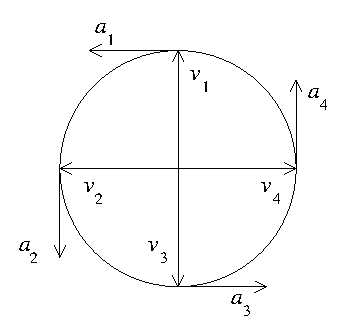
\includegraphics{speed_xfig}%
\end{picture}%
\setlength{\unitlength}{4144sp}%
%
\begingroup\makeatletter\ifx\SetFigFont\undefined%
\gdef\SetFigFont#1#2#3#4#5{%
  \reset@font\fontsize{#1}{#2pt}%
  \fontfamily{#3}\fontseries{#4}\fontshape{#5}%
  \selectfont}%
\fi\endgroup%
\begin{picture}(2386,2295)(661,-1651)
\end{picture}%
\caption{The speed of a turning object.}\label{fig:turning_object_speed}
\end{center}\end{figure}

The time to complete one revolution is still $T$. The change in velocity (acceleration) can be calculated by dividing the circumference of the circle by the rotation time:
\begin{equation}
a= \frac{2 \pi v}{T} \label{eq:a_T}
\end{equation}
Combining with equation~\ref{eq:T_v} yields:
\begin{equation}
a= \frac{2 \pi v}{\left( \frac{2 \pi r}{v}\right) } \label{eq:a_T_v}
\end{equation}
Or:
\begin{align}
a &= \frac{2 \pi v^2}{2 \pi r}\\
a &= \frac{v^2}{r}  \label{eq:a_v_r}
\end{align}
We know that:
\begin{equation}
 F = m \cdot a \tag{\ref{eq:newton2}}
\end{equation}
Substitution of equation~\ref{eq:newton2} into \ref{eq:a_v_r} gives:
\begin{equation}
F = \frac{m v^2}{r} \label{eq:centripetal1}
\end{equation}

A turning barrel rotates every point over the same angle in a certain amount of time. This means that the speed of a point is proportional to its radius (distance to the centre of the barrel). It is now convenient to introduce a new quantity: angular velocity $\omega$. The unit associated to angular velocity can be degrees per second, or radians per second. The relation between $v$ and $\omega$ is:
\begin{equation}
v = \omega r \label{eq:v_om_r}
\end{equation}
The centripetal force in equation~\ref{eq:centripetal1} can now be written as:
\begin{equation}
F = m \omega^2 r \label{eq:F_m_om_r}
\end{equation}

Now we can sketch how forces act on a particle on a rotating liquid surface; we have a force directed upwards and the centripetal force directed towards the centre of the barrel: figure~\ref{fig:forces_particle} (gravity is not depicted in the figure).

\begin{figure}\begin{center}
\begin{picture}(0,0)%
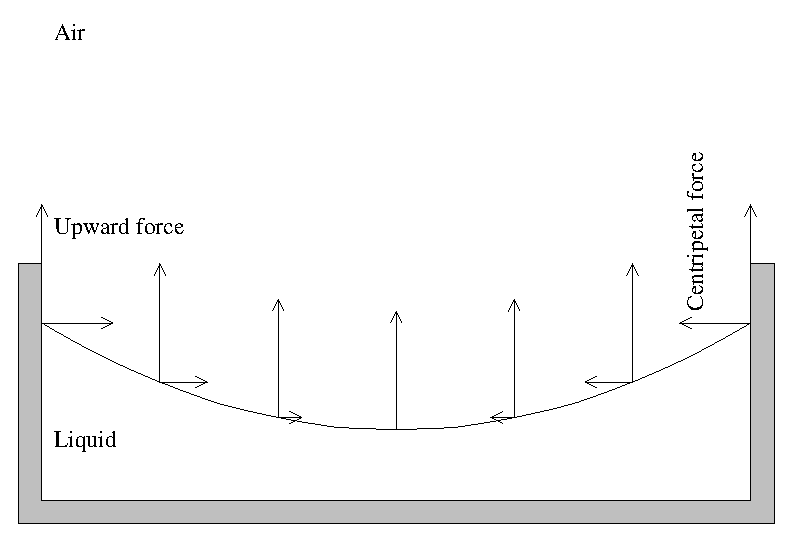
\includegraphics{glass_xfig}%
\end{picture}%
\setlength{\unitlength}{4144sp}%
%
\begingroup\makeatletter\ifx\SetFigFont\undefined%
\gdef\SetFigFont#1#2#3#4#5{%
  \reset@font\fontsize{#1}{#2pt}%
  \fontfamily{#3}\fontseries{#4}\fontshape{#5}%
  \selectfont}%
\fi\endgroup%
\begin{picture}(5784,3867)(-191,-1603)
\end{picture}%
\caption{Forces acting on a particle on a rotating surface.}\label{fig:forces_particle}
\end{center}\end{figure}

\begin{shaded}
\textbf{Exercise \theExercise \stepcounter{Exercise}} : Try to follow the derivation of the important equations of this section. Try to understand every consecutive step from equation to equation and how they describe the problem at hand.\end{shaded}
\begin{shaded}
\textbf{Exercise \theExercise \stepcounter{Exercise}} : Show that a turning liquid will obtain a parabolic surface.\end{shaded}

\section{Glass}
Spinning glass on a table does not make a mirror. All we have at this moment is a model to make a parabolic surface. If we were able to solidify the liquid while it has the parabolic shape we have the beginnings of a parabolic mirror. An entire barrel of glass will not solidify at once, certain parts of the barrel will be cooler than others. The cooler regions of the glass will solidify while others are still fluid. This causes tensions inside the glass. To keep the tensions to a minimum, and prevent the glass from braking, the liquid glass is cooled very slowly.

Window panes (sheets glass) are nowadays made with the Pinkerton process. In the Pinkerton Float Glass process liquid glass floats on a layer of liquid tin. The temperature of the tin is just below the melting point of glass, slowly cooling the hot glass. On one side of the tin bath new liquid glass is continuously poured onto the tin. On the other side of the bath the glass has completely solidified and can be taken out of the bath. Because this is a continuous process the panes of glass could, in principle, be infinitely long.

In a similar fashion liquid glass could be poured onto a spinning surface of tin. When the glass has cooled down and solidified it has the shape of a parabola. This process is difficult to be carried out at home or in school. But a similar experiment can be done with hot water and candle wax in a Petri dish on a turning table. 

\begin{shaded}
\textbf{Exercise \theExercise \stepcounter{Exercise}} : Try making a parabolic surface using water and candle wax. What materials do you need? How does the process work? What are the difficulties in making a parabolic surface? How do you overcome these difficulties? Make a report of your experiment.\end{shaded}
\begin{shaded}
\textbf{Exercise \theExercise \stepcounter{Exercise}} : Do a bit of (online) research: How is glass made?\end{shaded}

\end{document}